Grasp planning is an active area of research. In this paper we show how to plan (i) dexterous grasps, (ii) for novel objects, (iii) given a single view of each object. It is essentially this grasping problem which humans solve, so it is a high bar for robot grasping to reach. 

The combination of constraints makes the problem particularly challenging, because it means that surface reconstruction will be partial, yet this cannot be compensated for by fitting a known object model. This incompleteness in object surface reconstruction, together with additional uncertainty about object mass, co-efficients of friction, etcetera, renders infeasible the use of grasp planners that employ classical mechanics to predict grasp quality. Instead, we must employ a learning approach.

At the heart of reliable grasping there are two problems: generation and evaluation. Candidate grasps must be generated, and then each candidate must be evaluated, so as to produce one or more of a predicted grasp quality measure (e.g maximum resistable wrench), the probability of grasp success, the likely in-hand slip or rotation, etcetera. 
\begin{figure}[t]
  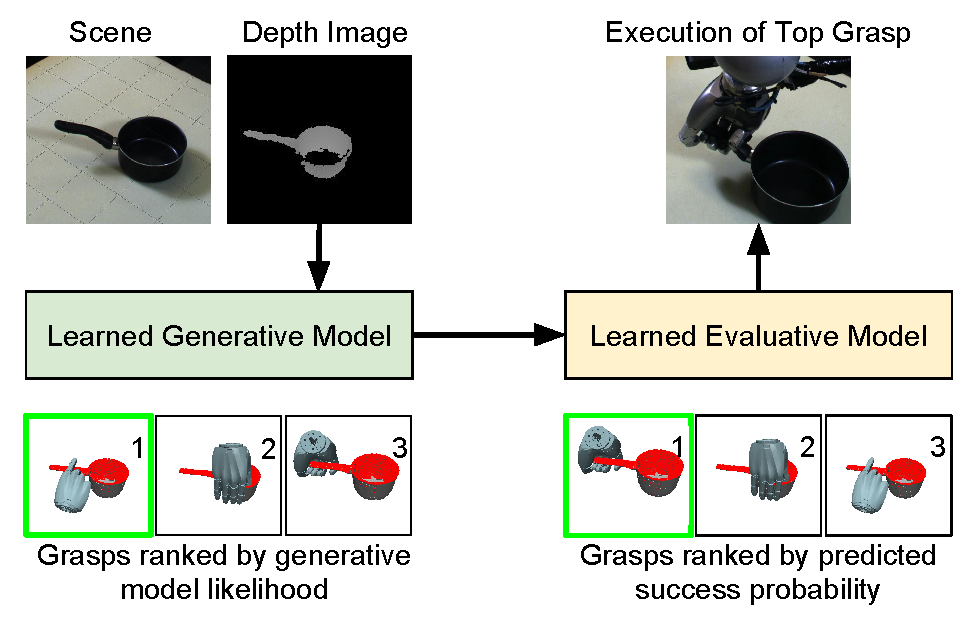
\includegraphics[width=\columnwidth]{images/contribution.pdf}
  \caption{The trained generative-evaluative architecture when presented with a novel object.}
\label{fig:systemArchitecture}
\end{figure}
Either or both a {\em generative} or {\em evaluative} model can be learned. If only a generative model is learned then evaluation must be carried out using mechanically informed reasoning, which cannot easily apply to our case of partial object reconstruction. If only an evaluative model is learned then grasp generation must proceed by search. This is feasible for pinch grippers, where the configuration space is of low dimension, but is more expensive for dexterous grasping, where the space can easily exceed 15 DoF. Thus, for dexterous grasping of novel objects from a single view it becomes appealing to learn both a generative and an evaluative model. This is the approach taken in this paper and it is, to the best of our knowledge, the first work to do so for dexterous grasping of novel objects from a single view.

Recently, data intensive learning methods have been shown to learn good evaluative models. %Levine predicts the probability of success for a possible pinch grasp constrained to lie in $SE(3)$, given an input image. Other work here ... 
But one restriction is that most of this work has only been applied to pinch grasping. (Before you say these are evaluative you have to re-read platt's latest papers to see exactly what they do). On the other hand, some data efficient methods for learning from demonstration (LfD) have recently been shown to learn good generative models.  
%may require fewer than ten example grasps. Some of these approaches learn {\em generative} models, and so can be used to generate many candidate grasps given an object. However, they are purely generative, so that there is no estimate of how probable the selected grasp is to succeed on a given object.

This paper combines the advantages of both approaches. A generative grasp model is learned from a small number of demonstrated grasps. Then an evaluative model is learned of the grasps generated by this model on new objects, using a deep neural network. To avoid a large data set of real grasps for training the evaluative model we exclusively use data generated by coupled sensor and rigid body simulations.
%This is used to generate grasps for simulated depth perception of objects. These candidate grasps are then are executed in a rigid body dynamics simulator. This allows a large enough virtual data set to be generated to train a data-intensive learner, in this case a deep neural network. The real robot is then possessed of a grasp generator, able to generate thousands of candidate grasps; and a grasp evaluator, which predicts the probability of a particular grasp succeeding and the grasp stability. 
To evaluate this generative-evaluative architecture a challenging test set of real object-pose pairs is used. 
%We select poses relative to camera pose that minimise the surface recovered by the depth camera. Although the method could be used when object reconstruction is nearly complete, we evaluate on the most challenging case of a single view.

The contributions of this paper are: i) the first combined generative-evaluative system for dexterous grasping of novel objects from a single view; ii) the configuration of sensor and rigid body simulations that enable a realistic data set to be generated, iii) an empirical study, showing that our architecture improves the success rate compared to the state of the art in dexterous grasping.

The paper is divided as follows. First, we discuss related work. Second, the  generative model is described. Third, we describe the design of the grasp simulation. Fourth, the architecture and training of the evaluative model is detailed. Fifth, we describe the experimental study, and then conclude.

